% Template for PLoS
% Version 3.6 Aug 2022
%
% % % % % % % % % % % % % % % % % % % % % %
%
% -- IMPORTANT NOTE
%
% This template contains comments intended 
% to minimize problems and delays during our production 
% process. Please follow the template instructions
% whenever possible.
%
% % % % % % % % % % % % % % % % % % % % % % % 
%
% Once your paper is accepted for publication, 
% PLEASE REMOVE ALL TRACKED CHANGES in this file 
% and leave only the final text of your manuscript. 
% PLOS recommends the use of latexdiff to track changes during review, as this will help to maintain a clean tex file.
% Visit https://www.ctan.org/pkg/latexdiff?lang=en for info or contact us at latex@plos.org.
%
%
% There are no restrictions on package use within the LaTeX files except that no packages listed in the template may be deleted.
%
% Please do not include colors or graphics in the text.
%
% The manuscript LaTeX source should be contained within a single file (do not use \input, \externaldocument, or similar commands).
%
% % % % % % % % % % % % % % % % % % % % % % %
%
% -- FIGURES AND TABLES
%
% Please include tables/figure captions directly after the paragraph where they are first cited in the text.
%
% DO NOT INCLUDE GRAPHICS IN YOUR MANUSCRIPT
% - Figures should be uploaded separately from your manuscript file. 
% - Figures generated using LaTeX should be extracted and removed from the PDF before submission. 
% - Figures containing multiple panels/subfigures must be combined into one image file before submission.
% For figure citations, please use "Fig" instead of "Figure".
% See http://journals.plos.org/plosone/s/figures for PLOS figure guidelines.
%
% Tables should be cell-based and may not contain:
% - spacing/line breaks within cells to alter layout or alignment
% - do not nest tabular environments (no tabular environments within tabular environments)
% - no graphics or colored text (cell background color/shading OK)
% See http://journals.plos.org/plosone/s/tables for table guidelines.
%
% For tables that exceed the width of the text column, use the adjustwidth environment as illustrated in the example table in text below.
%
% % % % % % % % % % % % % % % % % % % % % % % %
%
% -- EQUATIONS, MATH SYMBOLS, SUBSCRIPTS, AND SUPERSCRIPTS
%
% IMPORTANT
% Below are a few tips to help format your equations and other special characters according to our specifications. For more tips to help reduce the possibility of formatting errors during conversion, please see our LaTeX guidelines at http://journals.plos.org/plosone/s/latex
%
% For inline equations, please be sure to include all portions of an equation in the math environment.  For example, x$^2$ is incorrect; this should be formatted as $x^2$ (or $\mathrm{x}^2$ if the romanized font is desired).
%
% Do not include text that is not math in the math environment. For example, CO2 should be written as CO\textsubscript{2} instead of CO$_2$.
%
% Please add line breaks to long display equations when possible in order to fit size of the column. 
%
% For inline equations, please do not include punctuation (commas, etc) within the math environment unless this is part of the equation.
%
% When adding superscript or subscripts outside of brackets/braces, please group using {}.  For example, change "[U(D,E,\gamma)]^2" to "{[U(D,E,\gamma)]}^2". 
%
% Do not use \cal for caligraphic font.  Instead, use \mathcal{}
%
% % % % % % % % % % % % % % % % % % % % % % % % 
%
% Please contact latex@plos.org with any questions.
%
% % % % % % % % % % % % % % % % % % % % % % % %

\documentclass[10pt,letterpaper]{article}
\usepackage[top=0.85in,left=2.75in,footskip=0.75in]{geometry}

\usepackage{lscape}
\usepackage{colortbl}
\usepackage[table,xcdraw]{xcolor}
\usepackage{booktabs}



% amsmath and amssymb packages, useful for mathematical formulas and symbols
\usepackage{amsmath,amssymb}

% Use adjustwidth environment to exceed column width (see example table in text)
\usepackage{changepage}

% textcomp package and marvosym package for additional characters
\usepackage{textcomp,marvosym}

% cite package, to clean up citations in the main text. Do not remove.
\usepackage{cite}

% Use nameref to cite supporting information files (see Supporting Information section for more info)
\usepackage{nameref,hyperref}

% line numbers
\usepackage[right]{lineno}

% ligatures disabled
\usepackage[nopatch=eqnum]{microtype}
\DisableLigatures[f]{encoding = *, family = * }

% color can be used to apply background shading to table cells only
\usepackage[table]{xcolor}

% array package and thick rules for tables
\usepackage{array}

% create "+" rule type for thick vertical lines
\newcolumntype{+}{!{\vrule width 2pt}}

% create \thickcline for thick horizontal lines of variable length
\newlength\savedwidth
\newcommand\thickcline[1]{%
  \noalign{\global\savedwidth\arrayrulewidth\global\arrayrulewidth 2pt}%
  \cline{#1}%
  \noalign{\vskip\arrayrulewidth}%
  \noalign{\global\arrayrulewidth\savedwidth}%
}

% \thickhline command for thick horizontal lines that span the table
\newcommand\thickhline{\noalign{\global\savedwidth\arrayrulewidth\global\arrayrulewidth 2pt}%
\hline
\noalign{\global\arrayrulewidth\savedwidth}}


% Remove comment for double spacing
%\usepackage{setspace} 
%\doublespacing

% Text layout
\raggedright
\setlength{\parindent}{0.5cm}
\textwidth 5.25in 
\textheight 8.75in

% Bold the 'Figure #' in the caption and separate it from the title/caption with a period
% Captions will be left justified
\usepackage[aboveskip=1pt,labelfont=bf,labelsep=period,justification=raggedright,singlelinecheck=off]{caption}
\renewcommand{\figurename}{Fig}

% Use the PLoS provided BiBTeX style
\bibliographystyle{plos2015}

% Remove brackets from numbering in List of References
\makeatletter
\renewcommand{\@biblabel}[1]{\quad#1.}
\makeatother



% Header and Footer with logo
\usepackage{lastpage,fancyhdr,graphicx}
\usepackage{epstopdf}
%\pagestyle{myheadings}
\pagestyle{fancy}
\fancyhf{}
%\setlength{\headheight}{27.023pt}
%\lhead{\includegraphics[width=2.0in]{PLOS-submission.eps}}
\rfoot{\thepage/\pageref{LastPage}}
\renewcommand{\headrulewidth}{0pt}
\renewcommand{\footrule}{\hrule height 2pt \vspace{2mm}}
\fancyheadoffset[L]{2.25in}
\fancyfootoffset[L]{2.25in}
\lfoot{\today}

%% Include all macros below

\newcommand{\lorem}{{\bf LOREM}}
\newcommand{\ipsum}{{\bf IPSUM}}

%% END MACROS SECTION


\begin{document}
\vspace*{0.2in}

% Title must be 250 characters or less.
\begin{flushleft}
{\Large
\textbf\newline{Title of submission to PLOS journals} % Please use "sentence case" for title and headings (capitalize only the first word in a title (or heading), the first word in a subtitle (or subheading), and any proper nouns).
}
\newline
% Insert author names, affiliations and corresponding author email (do not include titles, positions, or degrees).
\\
Name1 Surname\textsuperscript{1,2\Yinyang},
Name2 Surname\textsuperscript{2\Yinyang},
Name3 Surname\textsuperscript{2,3\textcurrency},
Name4 Surname\textsuperscript{2},
Name5 Surname\textsuperscript{2\ddag},
Name6 Surname\textsuperscript{2\ddag},
Name7 Surname\textsuperscript{1,2,3*},
with the Lorem Ipsum Consortium\textsuperscript{\textpilcrow}
\\
\bigskip
\textbf{1} Affiliation Dept/Program/Center, Institution Name, City, State, Country
\\
\textbf{2} Affiliation Dept/Program/Center, Institution Name, City, State, Country
\\
\textbf{3} Affiliation Dept/Program/Center, Institution Name, City, State, Country
\\
\bigskip

% Insert additional author notes using the symbols described below. Insert symbol callouts after author names as necessary.
% 
% Remove or comment out the author notes below if they aren't used.
%
% Primary Equal Contribution Note
\Yinyang These authors contributed equally to this work.

% Additional Equal Contribution Note
% Also use this double-dagger symbol for special authorship notes, such as senior authorship.
\ddag These authors also contributed equally to this work.

% Current address notes
\textcurrency Current Address: Dept/Program/Center, Institution Name, City, State, Country % change symbol to "\textcurrency a" if more than one current address note
% \textcurrency b Insert second current address 
% \textcurrency c Insert third current address

% Deceased author note
\dag Deceased

% Group/Consortium Author Note
\textpilcrow Membership list can be found in the Acknowledgments section.

% Use the asterisk to denote corresponding authorship and provide email address in note below.
* correspondingauthor@institute.edu

\end{flushleft}
% Please keep the abstract below 300 words
\section*{Abstract}
Lorem ipsum dolor sit amet, consectetur adipiscing elit. Curabitur eget porta erat. Morbi consectetur est vel gravida pretium. Suspendisse ut dui eu ante cursus gravida non sed sem. Nullam sapien tellus, commodo id velit id, eleifend volutpat quam. Phasellus mauris velit, dapibus finibus elementum vel, pulvinar non tellus. Nunc pellentesque pretium diam, quis maximus dolor faucibus id. Nunc convallis sodales ante, ut ullamcorper est egestas vitae. Nam sit amet enim ultrices, ultrices elit pulvinar, volutpat risus.


% Please keep the Author Summary between 150 and 200 words
% Use first person. PLOS ONE authors please skip this step. 
% Author Summary not valid for PLOS ONE submissions.   
\section*{Author summary}
Lorem ipsum dolor sit amet, consectetur adipiscing elit. Curabitur eget porta erat. Morbi consectetur est vel gravida pretium. Suspendisse ut dui eu ante cursus gravida non sed sem. Nullam sapien tellus, commodo id velit id, eleifend volutpat quam. Phasellus mauris velit, dapibus finibus elementum vel, pulvinar non tellus. Nunc pellentesque pretium diam, quis maximus dolor faucibus id. Nunc convallis sodales ante, ut ullamcorper est egestas vitae. Nam sit amet enim ultrices, ultrices elit pulvinar, volutpat risus.

\linenumbers

% Use "Eq" instead of "Equation" for equation citations.
\section*{Introduction}
Lorem ipsum dolor sit~\cite{bib1} amet, consectetur adipiscing elit. Curabitur eget porta erat. Morbi consectetur est vel gravida pretium. Suspendisse ut dui eu ante cursus gravida non sed sem. Nullam Eq~(\ref{eq:schemeP}) sapien tellus, commodo id velit id, eleifend volutpat quam. Phasellus mauris velit, dapibus finibus elementum vel, pulvinar non tellus. Nunc pellentesque pretium diam, quis maximus dolor faucibus id.~\cite{bib2} Nunc convallis sodales ante, ut ullamcorper est egestas vitae. Nam sit amet enim ultrices, ultrices elit pulvinar, volutpat risus.

\begin{eqnarray}
\label{eq:schemeP}
	\mathrm{P_Y} = \underbrace{H(Y_n) - H(Y_n|\mathbf{V}^{Y}_{n})}_{S_Y} + \underbrace{H(Y_n|\mathbf{V}^{Y}_{n})- H(Y_n|\mathbf{V}^{X,Y}_{n})}_{T_{X\rightarrow Y}},
\end{eqnarray}

\section*{Materials and methods}

\subsection{Overview}


We conducted an offline/online BCI experiment, recording the EEG (Unicorn gtec – 8 Channels) from 29 right-handed participants (14 female; mean age = 22) during a single recording session. The experiment aims to study the feasibility of using Action Words (AW) as a paradigm for BCI, comparing this with the traditional Motor Imagery (MI) and Motor Observation (MO) paradigms. The tasks for MI consist of imaging right-hand or leg movement, while that for AW is reading and mentally rehearsing the presented arm and leg-related action words, and for MO is watching the corresponding first-person perspective videos of the action words. Participants completed two offline and one online run of each experimental condition (MO, MI, AW), in a counterbalanced order. Each run consisted of 30 trials (10 for online runs) with a trial duration of 9 seconds (offline) or 10 seconds (online with neurofeedback). We collected the Vividness of Movement Imagery Questionnaire-2 (VMIQ-2) and demographic information before the experiment. After the second run of each experimental condition, we collected NASA-TLX. At the end of the experiment, we asked usability questions about each condition. We evaluated the aforementioned paradigms using  Movement-Related Potentials (MRP), Event-Related Spectral Perturbation (ERSP), classification rates (offline and online), NASA-TLX, and usability questionnaires. The experiment was approved by the Ethics Commission from both Potsdam University and Institution University of Envigado.


\subsection{Participants}
We collected EEG data from 29 healthy and right-handed participants (14 female) in a voluntary manner. They were Spanish speakers, mostly engineering students (only one lecturer, one lawyer, and one professional in marketing and business) from the Institution University of Envigado, Colombia. Their ages range from 18 to 30 years old (mean= 21.89, SD=3.91). All of them reported normal or corrected to normal vision. None of them reported neurological or psychiatric disorders or drug abuse. No one had previous experience using BCI; only one person had previously used EEG for other purposes. Participants were informed both orally and in writing about the procedure and the EEG recording. All participants gave written informed consent.

\subsection{Materials}

The Lancaster Sensorimotor Norms represent a set of sensorimotor strength evaluation from 39,707 concepts across six perceptual modalities (touch, hearing, smell, taste, vision, and interoception) and five action effectors (mouth/throat, hand/arm, foot/leg, head excluding mouth/throat, and torso), collected from a total of 3,500 individual participants (cite lancaster). We initially chose the set of 25 high-ranked words using the foot/leg and hand/arm action effect. Later, we selected the five most prominent and adequate for the current setup, considering that for Motor Observation, we planned to reproduce the action words in a first-person perspective video. Therefore, we selected the words (Spanish version in parentheses)  "Write" (\textit{Escribir}), "Throw" (\textit{Lanzar}), "Cut" (\textit{Cortar}), "Plug" (\textit{Conectar}), "Clap" (\textit{Aplaudir}) for hand/arm, and  "Walk" (\textit{Caminar}), "Sit" (\textit{Sentar}), "Step" (\textit{Paso}), "Jump" (\textit{Saltar}), "Kick" (\textit{Patear}) for foot/leg. Figure \ref{sensorimotor_lancaster} shows the average ratings of Leg and Hand selected words from the Action, Perceptual, and Sensorimotor dimensions. We can perceive that in Action, the selected words reached over 4.0 in the corresponding factor; the ratings are similar for visual in the Perceptual and Sensorimotor, where similarly, like in Action, they reached over or close to 4.0 rating. This guarantees that these words represent a motor-related action and sensorimotor activity for each member, which will be crucial for the classification in BCI. 

The English selected Action Words were translated into Spanish, where words like "Plug" and "Step" were adapted to the video's activity. For pluging, its more close word is "connect", which translates "Conectar", and similarly with Step, the more similar movement is "Marching" (upping and down the knees), where in Spanish translates as "Marchar".  We recorded videos from a first-person perspective as Angelini and colleagues reported that the strongest sensorimotor responsiveness emerged from this perspective (cite). Additionally, we recorded these videos using different environments and persons executing the action, to generalize the action and user can not be distracted or overthink about the details around. Thus, a total of six videos for each AW were recorded for each limb (Legs and Hands). Also, the recording system (cameras) was different, but it kept high-quality videos. Some FP videos were affected by the natural movement of the body when it executes the actions. Finally, we created gender-matched videos to use with either women or men participants. The videos are available online at \href{https://drive.google.com/drive/folders/1tBw2gumuGx_a9fdr_oX_tJngc04v0xCf}{this link}. (This will be updated for the OSF repository link). For Motor Imagery, we used arrows to indicate either arm (upward) or leg (downward) imaginary movement.



\begin{figure}[!h]

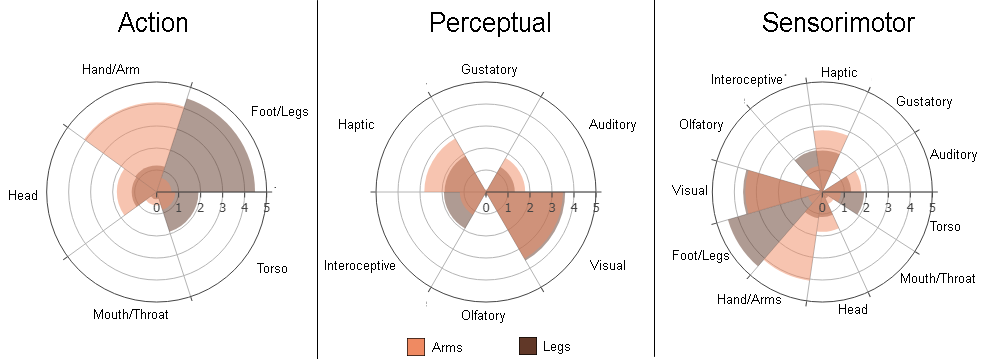
\includegraphics[width=\textwidth]{Figures/sensorimotor_plot.png}
\caption{{\bf Sensorimotor Lancaster Norms ratings.}
 Average ratings for the selected Arm and Leg Action Words. These ratings are represented in three dimensions: Action, Perceptual, and Sensorimotor. The average ratings evidence a clear distinction between Arm and Leg words for action and sensorimotor, and being similarly rated for visual in Perceptual and Sensorimotor. }
\label{sensorimotor_lancaster}
\end{figure}



\subsection{Procedure}


The subjects sat and were asked to make themselves comfortable and avoid any other movements during the recordings. The experiment ran on a laptop computer placed at 60-80 cm from the subject.

Our main objective is to check the feasibility of using Action Words instead of Motor Imagery or Motor Observation for BCI. To test this, we asked the subjects to perform right-hand and leg imaginary movement in each paradigm accordingly to the stimuli. Action words are presented at the center of the screen in Arial, white color with black as background, and a visual angle of approximately 3.0 to 6.0 degrees. Videos were presented in the middle of the screen with a resolution of 800x800 pixels. Similarly, cross and arrows for Motor Imagery were placed in the middle, rendered in white color. We used Psychopy 2023 to visualize the stimuli. We had two experiment modes: offline and online. During online, we presented the accuracy percentage as neurofeedback. Following Alimardini and colleagues (cite), who demonstrated that positive-biased leads to higher self-regulation motor imagery brain patterns, we include pseudo-random feedback based on the real accuracy + number generator from 0-20, keeping the upper limits of a real accuracy value (below 100). Both modes shared the same experimental protocol, with online including the feedback part (2 secs more). Each trial began with a black screen for 3 seconds, followed by the attention cue where a cross fixation appears and a beep sound is reproduced by 1 - 1.5 secs. Later, the motor cue is presented for three seconds: either the Action Word (AW), the arrow and cross fixation (Motor Imagery), or the video (Motor Observation). After this, during online, the feedback appears for 2 secs, and then the trial ends with 1.0 to 1.5 secs for inter-trial interval (Fig \ref{timing_protocol}).

For AW, Participants were instructed to read mentally the word and rehearsal the motor action. While for MO, merely observing the video. And for MI, following Neuper et al.~\cite{Neuper38}, we encouraged the subjects to perform the kinesthetic experience strategy during the execution of the imagery tasks, as this showed better performance in the classifiers. Participants completed two offline and one online runs of each experimental condition (MO, MI, AW) in a counterbalanced order. Each run consisted of 20 trials (10 for online runs) with a trial duration of 9 seconds (offline) or 12 seconds (online with neurofeedback). Between each run, a resting period of 5 minutes took place. 
The participants filled up demographics and Vividness of Movement Imagery Questionnaire-2 (VMIQ-2) at the beginning. Later, after the second run of each paradigm, they completed the NASA-TLX. Finally, subjective and usability questions were asked in a final questionnaire. 

\begin{figure}[!h]
 \centering
 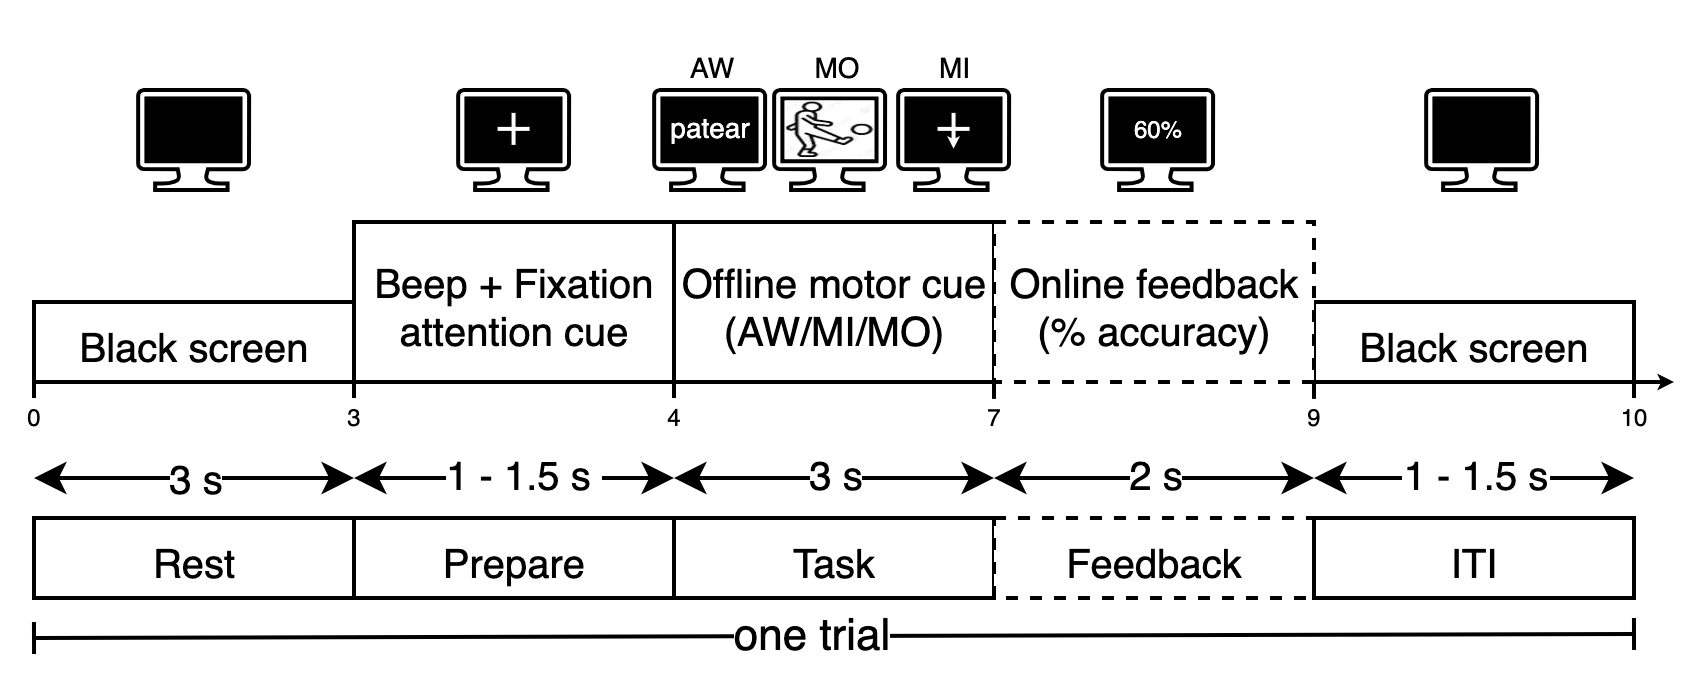
\includegraphics[width=\textwidth]{Figures/BCI_AW_MI_MO.png}
\caption{{\bf Experimental timing.}
The trial is composed of three seconds for resting (gray screen), 1.0 to 1.5 seconds for preparing (a beep sound plus the visual cue), followed by three seconds for performing the task (motor action), plus two seconds for feedback (only for online), and finally an inter-trial interval for 1.0 to 1.5 seconds. In total, each trial lasts nine seconds for offline and 10 for online.}
 \label{timing_protocol}
\end{figure}

 
\subsection{Data Acquisition and Analysis}

\subsubsection{Apparatus}

We collected the EEG data using a g.tec Unicorn Hybrid Black 24-bit board at a sampling rate of 250 Hz. Following the 10-20 EEG placement system, eight hybrid electrodes were used and placed on the scalp over areas that cover the Frontal (Fz), Central (C3, Cz, C4), Parietal (PO7, Pz, PO8), and Occipital (Oz) cortices. Left and right mastoids were used as reference and ground electrodes, respectively. Labstreaminglayer (LSL) is used for recording and synchronizing the EEG data with Psychopy.


\subsubsection{Signal processing}

We used EEGLAB (2024.2.1) \cite{delorme46} under Matlab 2023b to process the raw EEG data. The initial processing steps involved loading the data and removing epochs and events that were not part of the experimental conditions (Arm and Leg). We applied a band-pass filter from 1 to 40 Hz using a finite impulse response (FIR) filter. Line noise at 60 Hz was addressed using the Cleanline plugin to avoid the creation of band-holes and distortions that can occur with notch filters. The data was then re-referenced using a common average reference (CAR). Artifact rejection was performed using the Cleanraw plugin with specific criteria (BurstCriterion=25, WindowCriterion=0.2) to automatically identify and remove corrupted data segments. The percentage of retained data and the variance reduction in decibels (dB) from this process were calculated and stored for each participant. After this procedure, in average, 17\% of Arm events were rejected while 18\% of Legs events. This data processing stage aligns with the principles of Makoto's EEGLAB pipeline for EEG data processing.\cite{makotopipeline}

\subsubsection{Feature Extraction and Classification}

This study integrates two distinct types of electroencephalography (EEG) features: Event-Related Potentials (ERP) and oscillatory activity, characterized by Event-Related de-Synchronization/Synchronization (ERD/ERS) and analyzed through Filter Bank Common Spatial Pattern (FBCSP) features. While ERD/ERS patterns are commonly used in Motor Imagery (MI) Brain-Computer Interfaces (BCIs) to capture changes in alpha and beta frequency bands, ERPs are stimulus-locked components that provide additional temporal information. The inclusion of Action Words as a paradigm introduces both of these components, making it beneficial to analyze both stimulus-locked and time-locked EEG signals to comprehensively evaluate the neural response and improve classification accuracy.

ERP features were extracted from a specific set of channels, including Fz, C3, Cz, C4, Pz, and Oz. This was done on epochs with a time window from -0.5s to 2.5s relative to the cue, using a baseline correction from -0.5s to 0s. The features were computed as the mean amplitude within a sliding window of 0.5s with a step size of 0.5s. As a result, we had 36 features (6 time windows x 6 channels). FBCSP features were extracted from channels C3, Cz, C4, PO7, Pz, and PO8. The signal was filtered into multiple frequency bands: 8-12 Hz, 12-16 Hz, 16-20 Hz, 20-24 Hz, 24-28 Hz, and 13-30 Hz. The spatial patterns were then computed using CSP on a time window from 0.5s to 3.0s after the cue. As a result, we had 24 features (6 filter bands x 4 CSP components). To reduce the dimensionality and improve separability, mRMR (minimum Redundancy Maximum Relevance) feature selection was applied to both ERP and FBCSP feature sets, selecting the top 10 features for each. Before feature selection, the features were scaled using a StandardScaler.


Then, we used a Support Vector Machine (SVC) with a linear kernel (no hyperparameterization) to distinguish leg and arm signals. The model's performance was evaluated for each of the three paradigms (AW, MI, MO) using three different feature sets: i) only FBCSP features; ii) only ERP features; and iii) a combined feature set of both FBCSP and ERP features. The classification was carried out in two phases: offline and online. Offline classification uses A 10-fold stratified cross-validation on the offline data to assess the performance of each model configuration. While online classification uses the models trained on the offline data to classify unseen online epochs. We simulate an online scenario using an over-time classification, where the classifier was applied to a 2.5s sliding window with a step size of 0.25s over a 5s period of the online data. For Action Words, the online performance was further analyzed by differentiating between "seen" words (those present in the offline training set) and "new" words (not present in the offline training set). This represents a real generalization because most Motor Imagery BCI systems use the same cue during offline and online, where the classifiers reproduce a memorization task instead of predicting new unseen data.

\subsubsection{Movement-related Potential and Event-related spectral perturbation}


To effectively analyze the neurophysiological correlates of the three paradigms, we conducted two distinct but complementary analyses. Motor Imagery (MI) is traditionally associated with modulations of oscillatory activity in the alpha (8-12 Hz) and beta (13-30 Hz) frequency bands, known as Event-Related Desynchronization/Synchronization (ERD/ERS) patterns. However, paradigms involving linguistic processing, such as Action Words (AW), have been shown to elicit both these oscillatory patterns and time-locked temporal components, known as Event-Related Potentials (ERPs). Therefore, examining both spectral and temporal responses provides a more comprehensive understanding of the neural activity elicited by each task. It is important to note that the term Movement-Related Potential (MRP) is also used to refer to the temporal components preceding and accompanying movements. In this context, our ERP analysis serves to capture these temporal dynamics.

The initial step for both analyses involved segmenting the cleaned data into epochs based on the visual cue for either arm or leg movements. These epochs, spanning from -1000 ms to 3000 ms relative to the cue, were then grouped by paradigm (AW, MO, MI) and task (arm or leg) for further processing. The Event-Related Spectral Perturbation (ERSP) was calculated using the newtimef function in EEGLAB. This analysis was performed on the C3, Cz, and C4 electrodes, which are located over the sensorimotor cortex. The function computed the changes in spectral power in a time-frequency domain for a frequency range of 4-40 Hz and a time window of -1000 ms to 3000 ms relative to the cue. A baseline correction was applied using the interval from -1000 ms to 0 ms. For each condition, the data from all subjects and trials were merged to generate a grand average ERSP.

Event-Related Potentials (ERPs) were computed in the time domain for a broader set of channels: Fz, C3, Cz, C4, Pz, and Oz. For each subject and condition, all trial epochs were averaged to generate an ERP waveform. A baseline correction was applied using the time window from -500 ms to 0 ms. Finally, a grand average ERP was calculated by averaging the ERPs across all subjects to examine the overall temporal brain response for each task. A moving average with a window of 10 samples was then applied to the ERP waveform to smooth the data.


\subsection{Vividness of Movement Imagery Questionnaire-2 (VMIQ-2) and NASA Task Load Index}

Vividness of Movement Imagery Questionnaire-2 (VMIQ-2) is a self-report scale designed to measure a person's ability to vividly imagine themselves performing simple motor tasks. The questionnaire assesses three distinct types of imagery on a 5-point Likert scale (1 = No image at all, 5 = Perfectly clear and as vivid as seeing it): internal visual imagery, external visual imagery, and kinesthetic imagery. The VMIQ-2 is an updated version of the original VMIQ, developed in 2008 by Roberts and colleagues. It consists of 36 items, with 12 items for each of the three subscales.
The VMIQ-2 is a practical tool for subjectively assessing a person's motor imagery capacity before they participate in motor imagery-based BCI experiments, as it can help identify individuals who might have difficulty with the task.

On the other hand, the NASA-TLX (Task Load Index) is a commonly used subjective method to measure perceived workload. It evaluates workload across six dimensions: Mental Demand, Physical Demand, Temporal Demand, Performance, Effort, and Frustration. Each of these dimensions is rated on a 10-point scale, with anchors ranging from "low" to "high" or "good" to "poor" for performance. In addition to the ratings, the NASA-TLX includes a pairwise comparison procedure. Participants are asked to identify which of the six dimensions contributed most to the overall workload of a task. The number of times a dimension is selected in these comparisons is used to weight its corresponding rating, resulting in a single, comprehensive workload score. 



% Results and Discussion can be combined.
\section*{Results}


\begin{figure}[!h]
 \centering
 \includegraphics[width=\textwidth]{Figures/AW_MI_MO_ARMS_ERSP.eps}
\caption{{\bf Experimental timing.}
The trial is composed of three seconds for resting (gray screen), 1.0 to 1.5 seconds for preparing (a beep sound plus the visual cue), followed by three seconds for performing the task (motor action), plus two seconds for feedback (only for online), and finally an inter-trial interval for 1.0 to 1.5 seconds. In total, each trial lasts nine seconds for offline and 10 for online.}
 \label{timing_protocol}
\end{figure}





Nulla mi mi, venenatis sed ipsum varius, Table~\ref{table1} volutpat euismod diam. Proin rutrum vel massa non gravida. Quisque tempor sem et dignissim rutrum. Lorem ipsum dolor sit amet, consectetur adipiscing elit. Morbi at justo vitae nulla elementum commodo eu id massa. In vitae diam ac augue semper tincidunt eu ut eros. Fusce fringilla erat porttitor lectus cursus, vel sagittis arcu lobortis. Aliquam in enim semper, aliquam massa id, cursus neque. Praesent faucibus semper libero.

% Place tables after the first paragraph in which they are cited.
\begin{table}[!ht]
\begin{adjustwidth}{-2.25in}{0in} % Comment out/remove adjustwidth environment if table fits in text column.
\centering
\caption{
{\bf Table caption Nulla mi mi, venenatis sed ipsum varius, volutpat euismod diam.}}
\begin{tabular}{|l+l|l|l|l|l|l|l|}
\hline
\multicolumn{4}{|l|}{\bf Heading1} & \multicolumn{4}{|l|}{\bf Heading2}\\ \thickhline
$cell1 row1$ & cell2 row 1 & cell3 row 1 & cell4 row 1 & cell5 row 1 & cell6 row 1 & cell7 row 1 & cell8 row 1\\ \hline
$cell1 row2$ & cell2 row 2 & cell3 row 2 & cell4 row 2 & cell5 row 2 & cell6 row 2 & cell7 row 2 & cell8 row 2\\ \hline
$cell1 row3$ & cell2 row 3 & cell3 row 3 & cell4 row 3 & cell5 row 3 & cell6 row 3 & cell7 row 3 & cell8 row 3\\ \hline
\end{tabular}
\begin{flushleft} Table notes Phasellus venenatis, tortor nec vestibulum mattis, massa tortor interdum felis, nec pellentesque metus tortor nec nisl. Ut ornare mauris tellus, vel dapibus arcu suscipit sed.
\end{flushleft}
\label{table1}
\end{adjustwidth}
\end{table}


%PLOS does not support heading levels beyond the 3rd (no 4th level headings).
\subsection*{\lorem\ and \ipsum\ nunc blandit a tortor}
\subsubsection*{3rd level heading} 
Maecenas convallis mauris sit amet sem ultrices gravida. Etiam eget sapien nibh. Sed ac ipsum eget enim egestas ullamcorper nec euismod ligula. Curabitur fringilla pulvinar lectus consectetur pellentesque. Quisque augue sem, tincidunt sit amet feugiat eget, ullamcorper sed velit. Sed non aliquet felis. Lorem ipsum dolor sit amet, consectetur adipiscing elit. Mauris commodo justo ac dui pretium imperdiet. Sed suscipit iaculis mi at feugiat. 

\begin{enumerate}
	\item{react}
	\item{diffuse free particles}
	\item{increment time by dt and go to 1}
\end{enumerate}


\subsection*{Sed ac quam id nisi malesuada congue}

Nulla mi mi, venenatis sed ipsum varius, volutpat euismod diam. Proin rutrum vel massa non gravida. Quisque tempor sem et dignissim rutrum. Lorem ipsum dolor sit amet, consectetur adipiscing elit. Morbi at justo vitae nulla elementum commodo eu id massa. In vitae diam ac augue semper tincidunt eu ut eros. Fusce fringilla erat porttitor lectus cursus, vel sagittis arcu lobortis. Aliquam in enim semper, aliquam massa id, cursus neque. Praesent faucibus semper libero.

\begin{itemize}
	\item First bulleted item.
	\item Second bulleted item.
	\item Third bulleted item.
\end{itemize}

\section*{Discussion}
Nulla mi mi, venenatis sed ipsum varius, Table~\ref{table1} volutpat euismod diam. Proin rutrum vel massa non gravida. Quisque tempor sem et dignissim rutrum. Lorem ipsum dolor sit amet, consectetur adipiscing elit. Morbi at justo vitae nulla elementum commodo eu id massa. In vitae diam ac augue semper tincidunt eu ut eros. Fusce fringilla erat porttitor lectus cursus, vel sagittis arcu lobortis. Aliquam in enim semper, aliquam massa id, cursus neque. Praesent faucibus semper libero~\cite{bib3}.

\section*{Conclusion}

CO\textsubscript{2} Maecenas convallis mauris sit amet sem ultrices gravida. Etiam eget sapien nibh. Sed ac ipsum eget enim egestas ullamcorper nec euismod ligula. Curabitur fringilla pulvinar lectus consectetur pellentesque. Quisque augue sem, tincidunt sit amet feugiat eget, ullamcorper sed velit. 

Sed non aliquet felis. Lorem ipsum dolor sit amet, consectetur adipiscing elit. Mauris commodo justo ac dui pretium imperdiet. Sed suscipit iaculis mi at feugiat. Ut neque ipsum, luctus id lacus ut, laoreet scelerisque urna. Phasellus venenatis, tortor nec vestibulum mattis, massa tortor interdum felis, nec pellentesque metus tortor nec nisl. Ut ornare mauris tellus, vel dapibus arcu suscipit sed. Nam condimentum sem eget mollis euismod. Nullam dui urna, gravida venenatis dui et, tincidunt sodales ex. Nunc est dui, sodales sed mauris nec, auctor sagittis leo. Aliquam tincidunt, ex in facilisis elementum, libero lectus luctus est, non vulputate nisl augue at dolor. For more information, see \nameref{S1_Appendix}.

\section*{Supporting information}

% Include only the SI item label in the paragraph heading. Use the \nameref{label} command to cite SI items in the text.
\paragraph*{S1 Fig.}
\label{S1_Fig}
{\bf Bold the title sentence.} Add descriptive text after the title of the item (optional).

% Please add the following required packages to your document preamble:
% \usepackage{booktabs}
% \usepackage{graphicx}
% \usepackage[table,xcdraw]{xcolor}
% Beamer presentation requires \usepackage{colortbl} instead of \usepackage[table,xcdraw]{xcolor}
\begin{table}[]
\caption{Linguistic features of action words in English and Spanish. }
\label{SM_table1}
\resizebox{\textwidth}{!}{%
\begin{tabular}{@{}lllllll@{}}
\toprule
\rowcolor[HTML]{EFEFEF} 
Word\_En & Word\_Sp & AW\_limb & Log\_freq\_En & Log\_freq\_Sp & Syllabes\_En (letters) & Syllabes\_Sp (letters) \\ \midrule
JUMP    & SALTAR   & Leg & 4.629 & 4.438 & 1 (4) & 2 (6) \\
\rowcolor[HTML]{EFEFEF} 
KICK    & PATEAR   & Leg & 4.514 & 3.595 & 1 (4) & 3 (6) \\
MARCH   & MARCHAR  & Leg & 4.960 & 4.235 & 1 (5) & 2 (7) \\
\rowcolor[HTML]{EFEFEF} 
SIT     & SENTAR   & Leg & 5.036 & 4.627 & 1 (3) & 2 (6) \\
WALK    & CAMINAR  & Leg & 5.089 & 4.858 & 1 (4) & 3 (7) \\
\rowcolor[HTML]{EFEFEF} 
CLAP    & APLAUDIR & Arm & 3.391 & 3.777 & 1 (4) & 3 (8) \\
CONNECT & CONECTAR & Arm & 4.368 & 4.740 & 2 (7) & 3 (8) \\
\rowcolor[HTML]{EFEFEF} 
CUT     & CORTAR   & Arm & 5.279 & 4.639 & 1 (3) & 2 (6) \\
THROW   & LANZAR   & Arm & 4.787 & 4.718 & 1 (4) & 2 (6) \\
\rowcolor[HTML]{EFEFEF} 
WRITE   & ESCRIBIR & Arm & 5.061 & 5.424 & 1 (4) & 3 (8) \\ \bottomrule
\end{tabular}%
}
\end{table}



% Please add the following required packages to your document preamble:
% \usepackage{booktabs}
% \usepackage{graphicx}
% \usepackage[table,xcdraw]{xcolor}
% Beamer presentation requires \usepackage{colortbl} instead of \usepackage[table,xcdraw]{xcolor}
\begin{table}[]
\caption{Linguistic features action words in }
\label{S_table2}
\resizebox{\textwidth}{!}{%
\begin{tabular}{@{}lllllllll@{}}
\toprule
\rowcolor[HTML]{EFEFEF} 
Word  & Foot\_leg (sd) & Hand\_arm (sd) & Head (sd)     & Mouth (sd)    & Torso (sd)    & Max\_strength & Exclusivity & Dominant  \\ \midrule
JUMP    & 4.85 (0.489)  & 1.7 (1.689)   & 1.3 (1.75)    & 0.3 (0.923)  & 2.55 (1.849)  & 4.85  & 0.425 & Foot\_leg \\
\rowcolor[HTML]{EFEFEF} 
KICK    & 4.75 (0.786)  & 0.15 (0.366)  & 0.55 (1.146)  & 0 (0)        & 0.65 (0.933)  & 4.75  & 0.779 & Foot\_leg \\
MARCH   & 3.6 (2.137)   & 1.55 (1.761)  & 1.35 (1.843)  & 0.55 (1.146) & 1.35 (1.899)  & 3.6   & 0.363 & Foot\_leg \\
\rowcolor[HTML]{EFEFEF} 
SIT   & 4.211 (0.976)  & 1.263 (1.593)  & 1.368 (1.571) & 0.263 (0.733) & 3.684 (1.701) & 4.211         & 0.366       & Foot\_leg \\
WALK    & 4.947 (0.229) & 1.368 (1.461) & 1.105 (1.243) & 0.526 (1.02) & 1.263 (1.368) & 4.947 & 0.48  & Foot\_leg \\
\rowcolor[HTML]{EFEFEF} 
CLAP    & 0.3 (0.923)   & 4.55 (1.05)   & 1.5 (2.013)   & 0.25 (0.639) & 0.55 (1.05)   & 4.55  & 0.601 & Hand\_arm \\
CONNECT & 0.75 (1.02)   & 2.3 (1.838)   & 1.8 (1.908)   & 1.25 (1.713) & 0.55 (1.276)  & 2.3   & 0.263 & Hand\_arm \\
\rowcolor[HTML]{EFEFEF} 
CUT     & 1.263 (1.727) & 4.211 (1.273) & 1.842 (1.922) & 1.053 (1.58) & 1.316 (1.668) & 4.211 & 0.326 & Hand\_arm \\
THROW & 0.864 (1.246)  & 4.591 (1.246)  & 1.545 (1.969) & 0.227 (0.869) & 1.409 (1.623) & 4.591         & 0.505       & Hand\_arm \\
\rowcolor[HTML]{EFEFEF} 
WRITE & 0.227 (0.752)  & 4.727 (0.703)  & 2.364 (2.06)  & 0.273 (0.767) & 0.409 (0.854) & 4.727         & 0.562       & Hand\_arm \\ \bottomrule
\end{tabular}%
}
\end{table}

% Please add the following required packages to your document preamble:
% \usepackage{booktabs}
% \usepackage{graphicx}
% \usepackage[table,xcdraw]{xcolor}
% Beamer presentation requires \usepackage{colortbl} instead of \usepackage[table,xcdraw]{xcolor}
\begin{table}[]
\caption{}
\label{Stable3}
\resizebox{\textwidth}{!}{%
\begin{tabular}{@{}llllllllll@{}}
\toprule
\rowcolor[HTML]{EFEFEF} 
Word & Auditory (sd) & Gustatory (sd) & Haptic (sd)   & Interoceptive (sd)            & Olfactory (sd) & Visual (sd)   & Max\_strength & Exclusivity & Dominant \\ \midrule
JUMP    & 1.556 (1.617) & 0 (0)         & 1.389 (1.787) & 2.833 (1.724) & 0 (0)         & 3.944 (1.392) & 3.944 & 0.406 & Visual   \\
\rowcolor[HTML]{EFEFEF} 
KICK    & 0.895 (1.15)  & 0.211 (0.631) & 3.526 (1.611) & 1.842 (1.608) & 0.158 (0.501) & 3.632 (1.461) & 3.632 & 0.338 & Visual   \\
MARCH   & 2.722 (1.776) & 0 (0)         & 0.611 (1.501) & 0.944 (1.474) & 0.278 (1.179) & 4.111 (1.676) & 4.111 & 0.474 & Visual   \\
\rowcolor[HTML]{EFEFEF} 
SIT  & 0.611 (1.337) & 0.194 (0.889)  & 2.306 (1.895) & 1.417 (1.888)\textbackslash{} & 0.222 (0.959)  & 3.194 (1.737) & 3.194         & 0.378       & Visual   \\
WALK    & 0.765 (1.437) & 0 (0)         & 1.588 (2.002) & 2.529 (1.807) & 0.176 (0.728) & 3.118 (1.965) & 3.118 & 0.381 & Visual   \\
\rowcolor[HTML]{EFEFEF} 
CLAP    & 4.625 (0.924) & 0 (0)         & 2.833 (1.880) & 0.625 (1.173) & 0 (0)         & 3.75 (1.294)  & 4.625 & 0.391 & Auditory \\
CONNECT & 1.158 (1.500) & 0.263 (0.733) & 1.579 (1.644) & 1.105 (1.595) & 0.211 (0.713) & 2.842 (2.218) & 2.842 & 0.368 & Visual   \\
\rowcolor[HTML]{EFEFEF} 
CUT     & 0.95 (1.276)  & 0.05 (0.224)  & 3.45 (1.820)  & 2.15 (2.134)  & 0.1 (0.308)   & 3.25 (1.773)  & 3.45  & 0.342 & Haptic   \\
THROW   & 1.059 (1.749) & 0 (0)         & 3 (1.936)     & 0.882 (1.536) & 0 (0)         & 4 (1.225)     & 4     & 0.447 & Visual   \\
\rowcolor[HTML]{EFEFEF} 
WRITE   & 1.116 (1.636) & 0.279 (1.054) & 3.163 (1.772) & 1.186 (1.763) & 0.256 (0.875) & 3.651 (1.771) & 3.651 & 0.352 & Visual   \\ \bottomrule
\end{tabular}%
}
\end{table}

% Please add the following required packages to your document preamble:
% \usepackage{booktabs}
% \usepackage{graphicx}
% \usepackage[table,xcdraw]{xcolor}
% Beamer presentation requires \usepackage{colortbl} instead of \usepackage[table,xcdraw]{xcolor}
\begin{table}[]
\caption{ta}
\label{SM_table}
\resizebox{\textwidth}{!}{%
\begin{tabular}{@{}lllllllllllllll@{}}
\toprule
\rowcolor[HTML]{EFEFEF} 
Word &
  Auditory (sd) &
  Gustatory (sd) &
  Haptic (sd) &
  Interoceptive (sd) &
  Olfactory (sd) &
  Visual (sd) &
  Foot\_leg (sd) &
  Hand\_arm (sd) &
  Head (sd) &
  Mouth (sd) &
  Torso (sd) &
  Max\_strength &
  Exclusivity &
  Dominant \\ \midrule
JUMP &
  1.556 (1.617) &
  0 (0) &
  1.389 (1.787) &
  2.833 (1.724) &
  0 (0) &
  3.944 (1.392) &
  4.85 (0.489) &
  1.7 (1.689) &
  1.3 (1.75) &
  0.3 (0.923) &
  2.55 (1.849) &
  4.85 &
  0.237 &
  Foot\_leg \\
\rowcolor[HTML]{EFEFEF} 
KICK &
  0.895 (1.15) &
  0.211 (0.631) &
  3.526 (1.611) &
  1.842 (1.608) &
  0.158 (0.501) &
  3.632 (1.461) &
  4.75 (0.786) &
  0.15 (0.366) &
  0.55 (1.146) &
  0 (0) &
  0.65 (0.933) &
  4.75 &
  0.29 &
  Foot\_leg \\
MARCH &
  2.722 (1.776) &
  0 (0) &
  0.611 (1.501) &
  0.944 (1.474) &
  0.278 (1.179) &
  4.111 (1.676) &
  3.6 (2.137) &
  1.55 (1.761) &
  1.35 (1.843) &
  0.55 (1.146) &
  1.35 (1.899) &
  4.111 &
  0.241 &
  Visual \\
\rowcolor[HTML]{EFEFEF} 
SIT &
  0.611 (1.337) &
  0.194 (0.889) &
  2.306 (1.895) &
  1.417 (1.888) &
  0.222 (0.959) &
  3.194 (1.737) &
  4.211 (0.976) &
  1.263 (1.593) &
  1.368 (1.571) &
  0.263 (0.733) &
  3.684 (1.701) &
  4.211 &
  0.214 &
  Foot\_leg \\
WALK &
  0.765 (1.437) &
  0 (0) &
  1.588 (2.002) &
  2.529 (1.807) &
  0.176 (0.728) &
  3.118 (1.965) &
  4.947 (0.229) &
  1.368 (1.461) &
  1.105 (1.243) &
  0.526 (1.02) &
  1.263 (1.368) &
  4.947 &
  0.285 &
  Foot\_leg \\
\rowcolor[HTML]{EFEFEF} 
CLAP &
  4.625 (0.924) &
  0 (0) &
  2.833 (1.880) &
  0.625 (1.173) &
  0 (0) &
  3.75 (1.294) &
  0.3 (0.923) &
  4.55 (1.050) &
  1.5 (2.013) &
  0.25 (0.639) &
  0.55 (1.05) &
  4.625 &
  0.244 &
  Auditory \\
CONNECT &
  1.158 (1.5) &
  0.263 (0.733) &
  1.579 (1.644) &
  1.105 (1.595) &
  0.211 (0.713) &
  2.842 (2.218) &
  0.75 (1.020) &
  2.3 (1.838) &
  1.8 (1.908) &
  1.25 (1.713) &
  0.55 (1.276) &
  2.842 &
  0.191 &
  Visual \\
\rowcolor[HTML]{EFEFEF} 
CUT &
  0.95 (1.276) &
  0.05 (0.224) &
  3.45 (1.820) &
  2.15 (2.134) &
  0.1 (0.308) &
  3.25 (1.773) &
  1.263 (1.727) &
  4.211 (1.273) &
  1.842 (1.922) &
  1.053 (1.58) &
  1.316 (1.668) &
  4.211 &
  0.212 &
  Hand\_arm \\
THROW &
  1.059 (1.749) &
  0 (0) &
  3 (1.936) &
  0.882 (1.536) &
  0 (0) &
  4 (1.225) &
  0.864 (1.246) &
  4.591 (0.796) &
  1.545 (1.969) &
  0.227 (0.869) &
  1.409 (1.623) &
  4.591 &
  0.261 &
  Hand\_arm \\
\rowcolor[HTML]{EFEFEF} 
WRITE &
  1.116 (1.636) &
  0.279 (1.054) &
  3.163 (1.772) &
  1.186 (1.763) &
  0.256 (0.875) &
  3.651 (1.771) &
  0.227 (0.752) &
  4.727 (0.703) &
  2.364 (2.06) &
  0.273 (0.767) &
  0.409 (0.854) &
  4.727 &
  0.255 &
  Hand\_arm \\ \bottomrule
\end{tabular}%
}
\end{table}




\paragraph*{S2 Fig.}
\label{S2_Fig}
{\bf Lorem ipsum.} Maecenas convallis mauris sit amet sem ultrices gravida. Etiam eget sapien nibh. Sed ac ipsum eget enim egestas ullamcorper nec euismod ligula. Curabitur fringilla pulvinar lectus consectetur pellentesque.

\paragraph*{S1 File.}
\label{S1_File}
{\bf Lorem ipsum.}  Maecenas convallis mauris sit amet sem ultrices gravida. Etiam eget sapien nibh. Sed ac ipsum eget enim egestas ullamcorper nec euismod ligula. Curabitur fringilla pulvinar lectus consectetur pellentesque.

\paragraph*{S1 Video.}
\label{S1_Video}
{\bf Lorem ipsum.}  Maecenas convallis mauris sit amet sem ultrices gravida. Etiam eget sapien nibh. Sed ac ipsum eget enim egestas ullamcorper nec euismod ligula. Curabitur fringilla pulvinar lectus consectetur pellentesque.

\paragraph*{S1 Appendix.}
\label{S1_Appendix}
{\bf Lorem ipsum.} Maecenas convallis mauris sit amet sem ultrices gravida. Etiam eget sapien nibh. Sed ac ipsum eget enim egestas ullamcorper nec euismod ligula. Curabitur fringilla pulvinar lectus consectetur pellentesque.

\paragraph*{S1 Table.}
\label{S1_Table}
{\bf Lorem ipsum.} Maecenas convallis mauris sit amet sem ultrices gravida. Etiam eget sapien nibh. Sed ac ipsum eget enim egestas ullamcorper nec euismod ligula. Curabitur fringilla pulvinar lectus consectetur pellentesque.

\section*{Acknowledgments}
Cras egestas velit mauris, eu mollis turpis pellentesque sit amet. Interdum et malesuada fames ac ante ipsum primis in faucibus. Nam id pretium nisi. Sed ac quam id nisi malesuada congue. Sed interdum aliquet augue, at pellentesque quam rhoncus vitae.

\nolinenumbers

% Either type in your references using
% \begin{thebibliography}{}
% \bibitem{}
% Text
% \end{thebibliography}
%
% or
%
% Compile your BiBTeX database using our plos2015.bst
% style file and paste the contents of your .bbl file
% here. See http://journals.plos.org/plosone/s/latex for 
% step-by-step instructions.
% 
\begin{thebibliography}{10}

\bibitem{bib1}
Conant GC, Wolfe KH.
\newblock {{T}urning a hobby into a job: how duplicated genes find new
  functions}.
\newblock Nat Rev Genet. 2008 Dec;9(12):938--950.

\bibitem{bib2}
Ohno S.
\newblock Evolution by gene duplication.
\newblock London: George Alien \& Unwin Ltd. Berlin, Heidelberg and New York:
  Springer-Verlag.; 1970.

\bibitem{bib3}
Magwire MM, Bayer F, Webster CL, Cao C, Jiggins FM.
\newblock {{S}uccessive increases in the resistance of {D}rosophila to viral
  infection through a transposon insertion followed by a {D}uplication}.
\newblock PLoS Genet. 2011 Oct;7(10):e1002337.

\end{thebibliography}



\end{document}

